\documentclass{unina_delivery_class}

\begin{document}

\color{TERTIARY}

% Title page

\pagecolor{TERTIARY}\afterpage{\nopagecolor}
\begin{titlepage}
  \begin{center}
    \vspace*{0.8cm}
    \Huge
    \textbf{\maintitle{}}

    \vspace*{0.5cm}

    \color{SECONDARY}
    \large
    \textbf{\authors{}}
    
    \vfill

    
\includegraphics[width=0.8\textwidth]{UninaDelivery_logo.png}
    
    \vfill

    \vspace*{0.5cm}
    
\includegraphics[width=0.7\textwidth]{DIETI_logo.pdf}
    \vspace*{-0.5cm}
  \end{center}
\end{titlepage}

% Table of contents
  \tableofcontents{}

% Chapters

  % Chapter 1 - "Analisi dei requisiti e progettazione del sistema"
  \chapter{Considerazioni sul Dominio}

\section{Analisi del Problema}

Si vuole progettare e sviluppare un database per la gestione della logistica delle spedizioni di merci.

Questo sistema deve essere in grado di gestire le informazioni relative ai clienti, ai mezzi di trasporto, ai corrieri, ai magazzini e ai prodotti, per poter essere a disposizione di un operatore incaricato alla pianificazione di spedizioni.

\section{Assunzioni sul Dominio} 

Per modellare il mini-mondo relativo al problema, si sono fatte le seguenti assunzioni:

\begin{itemize}
  \item \textbf{Il sistema gestisce spedizioni di merci presenti nei propri magazzini, verso clienti che hanno effettuato un ordine}.
  
  Si è assunto che la ditta a cui è rivolto il sistema non si occupi di spedizioni postali tra clienti, ma solo di spedizioni di merci presenti nei propri magazzini, che siano della ditta stessa o lasciate in gestione alla ditta da aziende terze.

  Quest'assunzione è stata fatta per avere una linea di continuità col requisito di controllo della disponibilità della merce, cosa di cui non si occupa un servizio postale.

  \item  \textbf{Il sistema si occupa della gestione delle spedizioni verso magazzini, oltre che verso clienti}.
  
  Si è assunto che la ditta a cui è rivolto il sistema possa avere la merce richiesta da un cliente distribuita in più magazzini, e che sia sconvenevole far partire spedizioni dirette verso il cliente da ogni magazzino che ha la merce richiesta.

  Si è quindi piuttosto presupposto un sistema di spedizioni intermedie per merci che non sono presenti nel magazzino più vicino al cliente, ma che sono presenti in altri magazzini della ditta.

  \item \textbf{Il sistema non si occupa di selezionare il percorso della merce dal magazzino originario al cliente}.
  
  Si è assunto che sia compito di un operatore  selezionare il percorso della merce dal magazzino originario al cliente, e che il sistema si occupi solo di gestire le informazioni relative alla spedizione.

  Si è quindi presupposto che una merce possa andare da un magazzino a potenzialmente qualsiasi altro, e che sarà premura di un operatore scegliere percorsi ragionevoli.

  Quest'assunzione è stata fatta in funzione del requisito della traccia che richiede di far gestire all'operatore la pianificazione delle spedizioni, che chiaramente comprende anche il percorso.

  \newpage
  \item \textbf{Struttura gerarchica dei magazzini}.
  
  Si è assunto, oltre alla presenza di molteplici magazzini di proprietà della ditta, che questi magazzini siano organizzati in una struttura gerarchica territoriale come segue:
  \begin{itemize}
    \item Ogni magazzino è \textbf{cittadino}, e può spedire direttamente ai clienti della sua città.
    \item Alcuni magazzini \textbf{cittadini} sono \textbf{regionali}, che smistano le merci in una regione.
    \item Alcuni magazzini \textbf{regionali} sono \textbf{nazionali}, che smistano le merci in una nazione.
    \item Alcuni magazzini \textbf{nazionali} sono \textbf{centrali}, che smistano le merci in un continente.
    \end{itemize}

  \item \textbf{Distribuzione mezzi di trasporto}.
  
  Si è assunto che la ditta abbia a disposizione diversi tipi e livelli di mezzi per il trasporto merci, e che questi mezzi siano distribuiti in maniera diversa fra i magazzini, in base alla loro dimensione e al loro ruolo nella struttura gerarchica.

  In particolare, si è deciso di dividere i mezzi di trasporto in:
  
  \begin{itemize}
    \item \textbf{Su strada}, come camion e furgoni, divisi a loro volta in:
      \begin{itemize}
        \item \textbf{Piccoli}, ovvero furgoncini, camion di piccole dimensioni e motocicli che possono essere guidati con una patente A o B, presenti in tutti i magazzini. Ogni mezzo \textbf{su strada piccolo} può coprire una zona comprendente diversi CAP, ed è impiegato in viaggi \textbf{cittadini e intraregionali} per raggiungere il cliente finale.
        \item \textbf{Grandi}, ovvero TIR e camion di grandi dimensioni, che possono essere guidati con una patente C, presenti in magazzini regionali o superiori, per il trasporto fra magazzini, in viaggi \textbf{interregionali e intranazionali}.
      \end{itemize}
    
    \item \textbf{Su ferro}, come treni e tram, presenti in magazzini nazionali o superiori, per il trasporto fra magazzini, in viaggi \textbf{internazionali e intracontinentali}.
    
    \item \textbf{Via acqua}, come navi, presenti solo nei magazzini centrali, per il trasporto fra magazzini, in viaggi \textbf{intercontinentali}.
    
    \item \textbf{Via aria}, come aerei, presenti solo nei magazzini centrali, per il trasporto fra magazzini, in viaggi \textbf{intercontinentali}.
  
  \end{itemize}

  \item \textbf{Gestione dei trasportatori}.
  
  Si è assunto che la ditta abbia diretta responsabilità solo sui mezzi su strada, e che i mezzi su ferro, via acqua e via aria siano di enti di spedizione terzi, con cui la ditta ha un contratto di collaborazione e per questo ne conserva solo l'eventuale disponibilità e i dati a essa relativi.

  Si è dunque presupposto che gli unici trasportatori dipendenti dalla ditta siano i conducenti dei mezzi su strada, dei quali il sistema terrà traccia, tra le altre cose, della tipologia di patente, per associarli ai mezzi che possono guidare.

  \item \textbf{Gestione di ordini e spedizioni}.
  
  Si è assunto che il cliente della ditta possa effettuare un ordine contenenti più prodotti, e che la ditta possa spedire i prodotti di un ordine in più spedizioni, in base alla disponibilità dei prodotti nei magazzini.

  Si è presupposto dunque che il sistema non si occupi di gestire le spedizione in modo da evitare ritardi sulle date di consegna, ma esclusivamente di presentare in ordine le spedizioni per permettere all'operatore che pianifica le spedizioni di scegliere percorsi che evitino ritardi.

\end{itemize}

% TODO: @zGenny UML and ER diagrams needs to be updated according to the new domain assumptions


  % Chapter 2 - "Progettazione del sistema"
  \chapter{Progettazione Concettuale}

\section{Premesse alla lettura dei diagrammi}

\subsection{Modelli Utilizzati}

Procediamo alla modellizzazione del mini-mondo, partendo dalla progettazione concettuale.

Questa fase di progettazione è stata svolta utilizzando, oltre che il modello \textbf{UML} nella forma di un \textbf{Class Diagram}, anche il modello \textbf{EER}, ovvero \textbf{Enhanced Entity Relationship}, per cogliere meglio aspetti del dominio che un modello \textbf{ER} classico non avrebbe potuto cogliere, come ad esempio \textbf{generalizzazioni e specializzazioni}.

\subsection{Precisazioni sui Diagrammi}

\subsubsection{EER Diagram}

Vista la densità del diagramma \textbf{EER}, si è deciso d'introdurre un \textbf{color coding} per facilitarne la lettura:

\begin{itemize}
  \item \textcolor{PRIMARY}{Entità}, e dunque Specializzazioni in \textcolor{PRIMARY}{arancione};
  \item \textcolor{CONTRAST}{Relazioni} in \textcolor{CONTRAST}{celeste};
  \item \textcolor{NEWGREEN}{Attributi} in \textcolor{NEWGREEN}{verde};
\end{itemize}

Inoltre, in caso di accavallamento di linee, si è deciso d'interrompere la linea in secondo piano in corrispondenza di un intersezione, così da evidenziare i diversi collegamenti.

\subsubsection{UML Class Diagram}

Per migliorare la leggibilità dei diagrammi, si è deciso di specificare le \textbf{molteplicità} degli attributi esclusivamente per sottolineare la possibilità di essere valorizzato a \textbf{NULL}. 

In tali casi si è utilizzata la molteplicità \textbf{[\(0..1\)]} esclusivamente per gli attributi di tipo \textbf{Bool}, mentre \textbf{[\(0..*\)]} per gli altri.

\bigskip

\begin{note}[Leggibilità dei Diagrammi]
  In caso di problemi di leggibilità dei diagrammi, sono disponibili le versioni originali nella pagina GitHub del progetto:
  \exlink{https://github.com/RiccardoElena/UninaDelivery/blob/develop/db/docs/sources/ER_Diagram.pdf}{ER Diagram} e \exlink{https://github.com/RiccardoElena/UninaDelivery/blob/develop/db/docs/sources/UML_Class_Diagram.pdf}{UML Class Diagram}.
\end{note}

\newpage
% TODO @zGenny export the ER diagram with the new changes and uncommend this part

\section{Enhanced Entity Relationship Diagram}
\begin{center}
  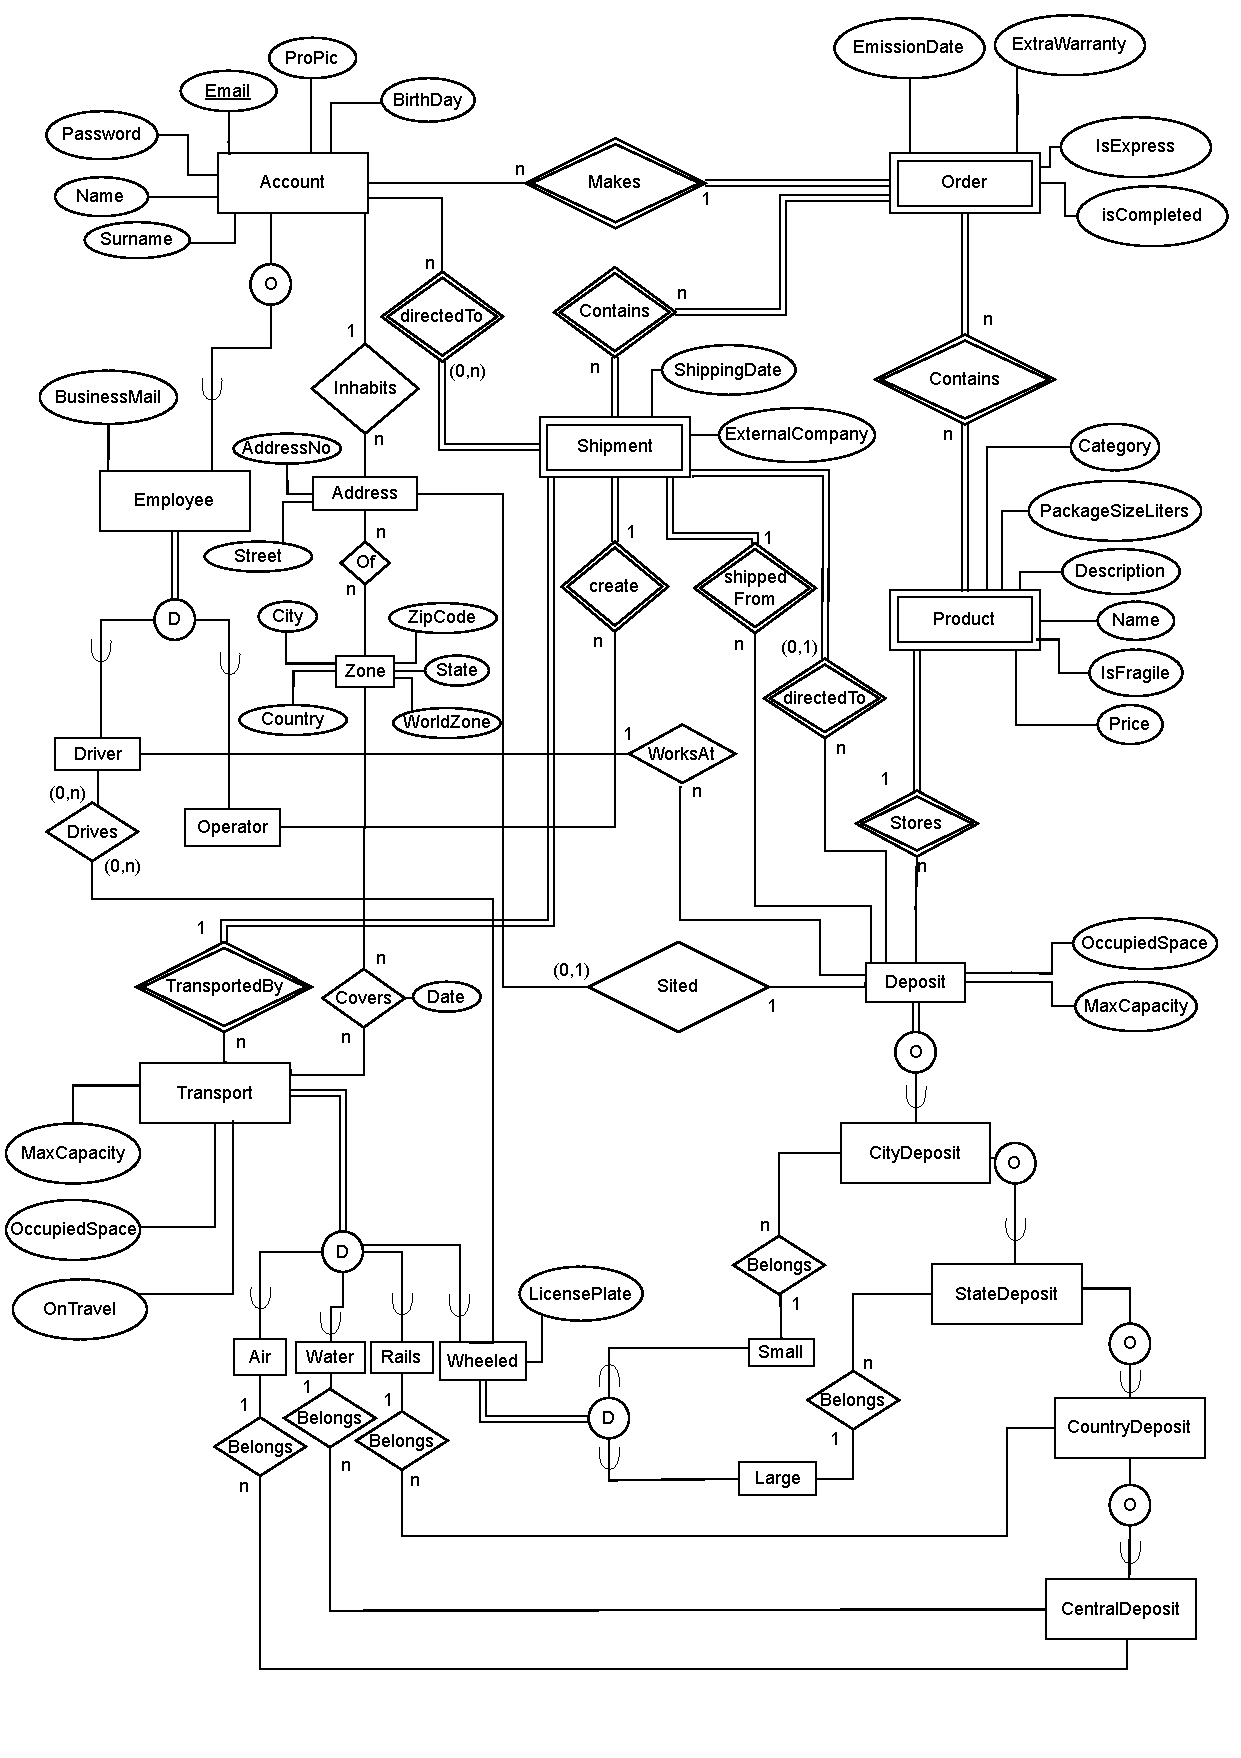
\includegraphics[width=0.9\textwidth]{ER_Diagram.pdf}
\end{center}

% TODO: need to re-export the UML diagram with the new changes. All the changes in the ER diagram are already done in the UML diagram
% If it's needed scale the size of the image with 0.x or 1.x near to \textwidth

\section{UML Class Diagram}
\begin{center}
  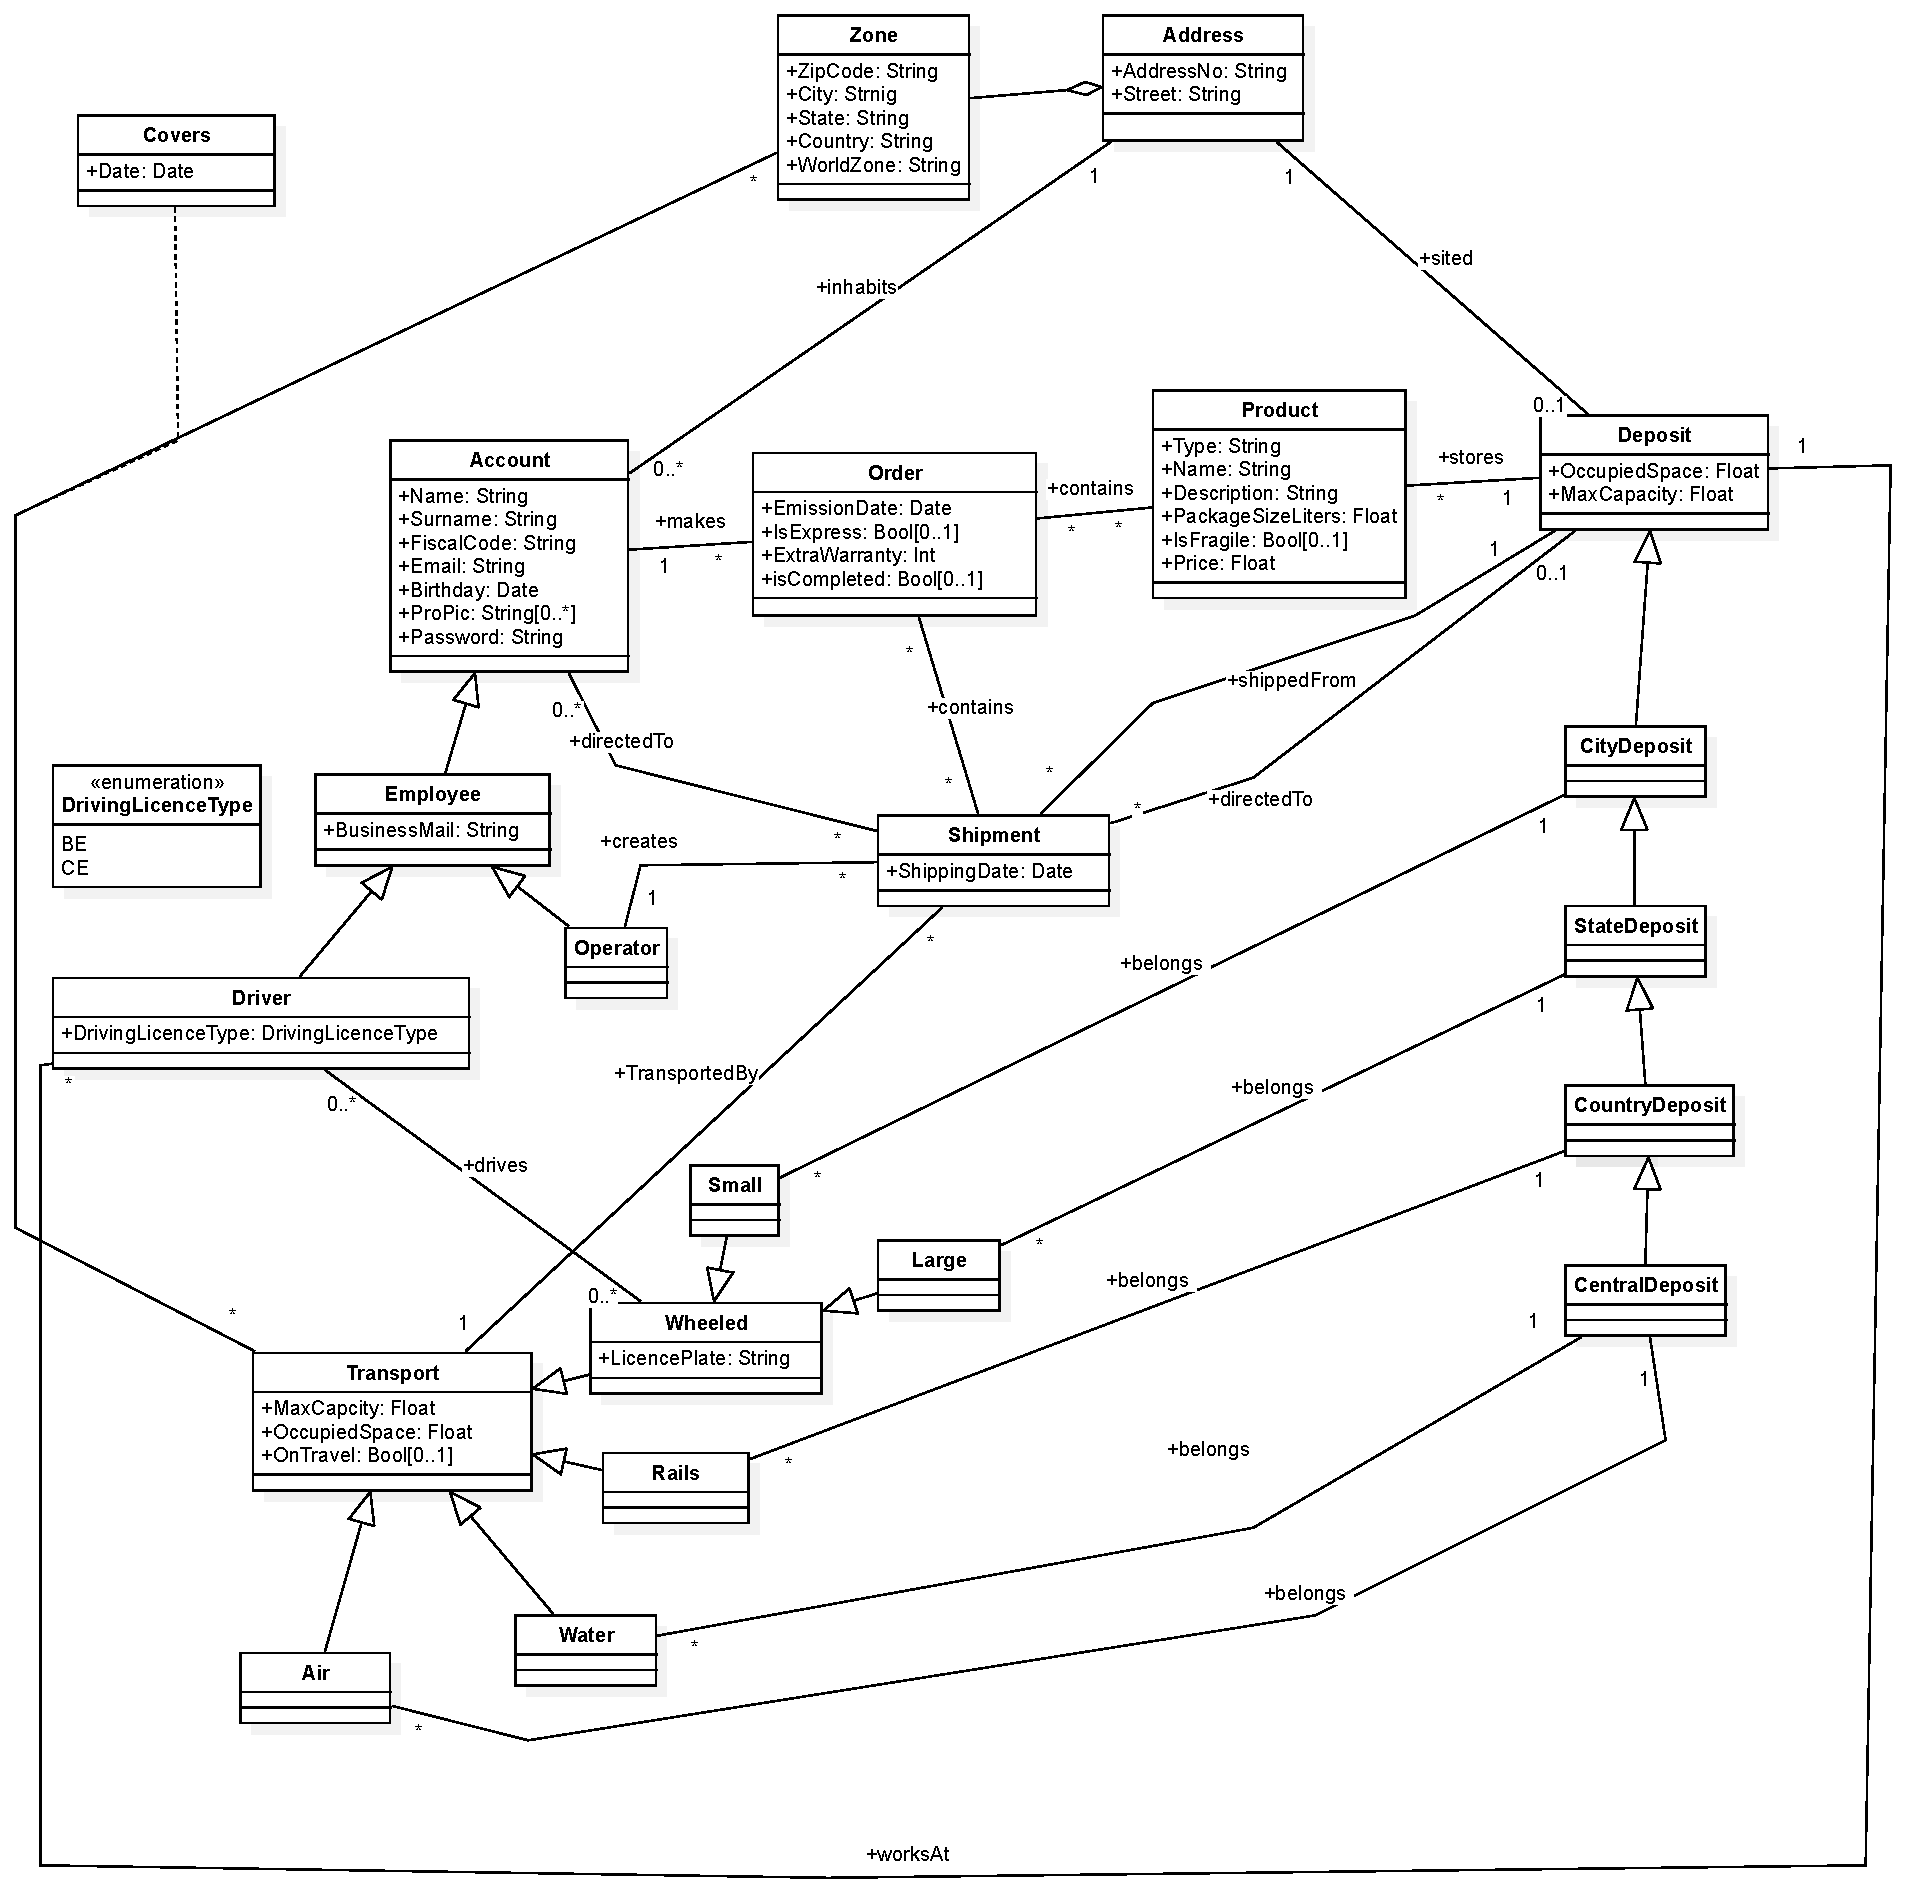
\includegraphics[width=\textwidth]{UML_Class_Diagram.pdf}
\end{center}

\newpage

\section{Ristrutturazione del Diagramma UML}

\subsection{Considerazioni sulla Ristrutturazione}

\subsubsection{Attributi Multipli e Multivalore}

Nello schema concettuale non sono presenti attributi \textbf{Multipli} o \textbf{Multivalore}, in quanto non sono stati ritenuti necessari per la rappresentazione del mini-mondo.

\subsubsection{Attributi Derivati}

Nello schema concettuale sono presenti due attributi \textbf{Derivati}:

\begin{itemize}
  \item L'attributo \textbf{Price} dell'entità \textbf{Shipment}, il quale però non ha necessità di essere conservato, non essendo un attributo di frequente richiesta per il sistema richiesto, e che quindi può essere eventualmente calcolato \textit{on-the-fly} in fase d'interrogazione del database basandosi sugli indirizzi di partenza e arrivo della spedizione e sulle eventuali modalità extra di consegna specificate in \textbf{Order}, come \textit{ExtraWarranty} e \textit{IsExpress}.
  \item L'attributo \textbf{IsCompleted} dell'entità \textbf{Order}, invece, si è scelto di conservarlo, in quanto è un attributo che può essere richiesto frequentemente dal sistema, e richiede un controllo relativamente complesso per essere valorizzato. Un ordine è considerato \textit{completato} se tutti i prodotti che contiene sono stati consegnati all'utente, dunque sarebbe necessario infatti controllare che tutti i prodotti dell'ordine siano stati spediti al destinatario, e che tali spedizioni siano andate a buon fine, coinvolgendo ben quattro entità: \textbf{Order}, \textbf{Product}, \textbf{Shipment} e \textbf{Account}. % * We should add a trigger that does this the first time
  \item L'attributo \textbf{OccupiedSpace} sia dell'entità \textbf{Deposit} che dell'entità \textbf{Transport}, infine, è stato anch'esso conservato, in quanto è un attributo che può essere richiesto frequentemente dal sistema, e richiede un interrogazione con risultato potenzialmente molto grande per essere valorizzata. % * this can be a cool trigger too.
\end{itemize}

\subsubsection{Generalizzazioni e Specializzazioni}

Le varie \textbf{Generalizzazioni} e \textbf{Specializzazioni} presenti nello schema concettuale sono state ristrutturate usando metodologie diverse, in base alla loro natura.

\begin{itemize}
  \item[\textbf{Employee:}] Essendo la specializzazione \textbf{Totale Disgiunta}, ed essendo le classi coinvolte in poche associazioni, si è scelto di accorpare la classe generale in quelle specializzate.
  \item[\textbf{Account:}] Essendo la specializzazione \textbf{Parziale Overlapping}, si è deciso di trasformarla in \textbf{Associazione}, limitando così il più possibile il numero di campi \textbf{NULL} e di \textbf{Vincoli d'Integrità}.
  \item[\textbf{Deposit:}] In questo caso trattandosi di una gerarchia di specializzazione si è scelto di accorpare a cascata le classi specializzate in quella generale, non avendo le classi specializzate attributi ed essendo tutte coinvolte in un'unica associazione concettualmente identica che verrà successivamente analizzata.
  \item[\textbf{Transport:}] Analogamente a quanto visto per \textbf{Deposit}, nonostante non si tratti di una gerarchia, si è scelto di accorpare le classi specializzate in quella generale. 
\end{itemize}

\subsubsection{Analisi delle Ridondanze}\label{Redundancy analysis}

Vediamo infine le ridondanze presenti nello schema concettuale, e come sono state rimosse.

Dalla ristrutturazione delle \textbf{Specializzazioni} di \textbf{Transport} sono emersi quattro attributi che servono essenzialmente lo stesso scopo ma per tipologie diverse di mezzi di trasporto: \textbf{Licence Plate}, \textbf{TrainNo}, \textbf{IMOCode} e \textbf{FlightNo}. Si è quindi deciso di accorpare questi attributi in un unico attributo \textbf{TransportID}, che può essere valorizzato con un identificativo univoco condiviso tra le tipologie di mezzi di trasporto, eliminando la possibilità di valori \textbf{NULL} o di valori uguali per tipi di mezzi diversi che imponevano aggiunta di vincoli o presenza di più attributi.

Inoltre la ristrutturazione delle \textbf{Specializzazioni} di \textbf{Deposit} ha fatto emergere quattro associazioni identiche a meno di vincoli che le riguardano, ovvero le associazioni \textbf{belongs}. È possibile dunque ridurle a un'unica associazione preservando i vincoli.

In ultima analisi, la classe \textbf{Shipment} è coinvolta in due associazioni semanticamente identiche, che si distinguono solo per molteplicità e seconda classe coinvolta, ovvero \textbf{Account} e \textbf{Deposit}. In particolare quella con \textbf{Account} è un'associazione circolare, essendo entrambe le classi associate anche con \textbf{Order}. Si è quindi deciso di eliminare l'associazione con \textbf{Account}, essendo il destinatario della spedizione già noto tramite \textbf{Order}.

\subsection{Identificazione delle Chiavi primarie}

Aldilà delle chiavi primarie già presenti nello schema concettuale esplicitate nel \textbf{diagramma ER} e dell'attributo \textbf{TransportID} introdotto \intlink{Redundancy analysis}{precedentemente}, si è deciso di aggiungere chiavi surrogate per le entità \textbf{Order}, \textbf{Shipment} e \textbf{Deposit}, poiché migrando le chiavi di altre entità si sarebbero ottenute chiavi composte troppo lunghe e complesse.

Per l'entità \textbf{Address} invece, è risultato più appropriato migrare la chiave primaria di \textbf{Zone} essendo una composizione e di conseguenza già concettualmente una \textit{parte} dell'entità \textbf{Address}. 

\newpage

\subsection{Class Diagram Ristrutturato}

% TODO: @zGenny review restructured diagram, if it's ok export it and uncommend this part. To adjust size add 0.x or 1.x near to \textwidth

% \begin{center}
  % ! USE THE NAME MENTIONED HERE FOR THE FILE
%   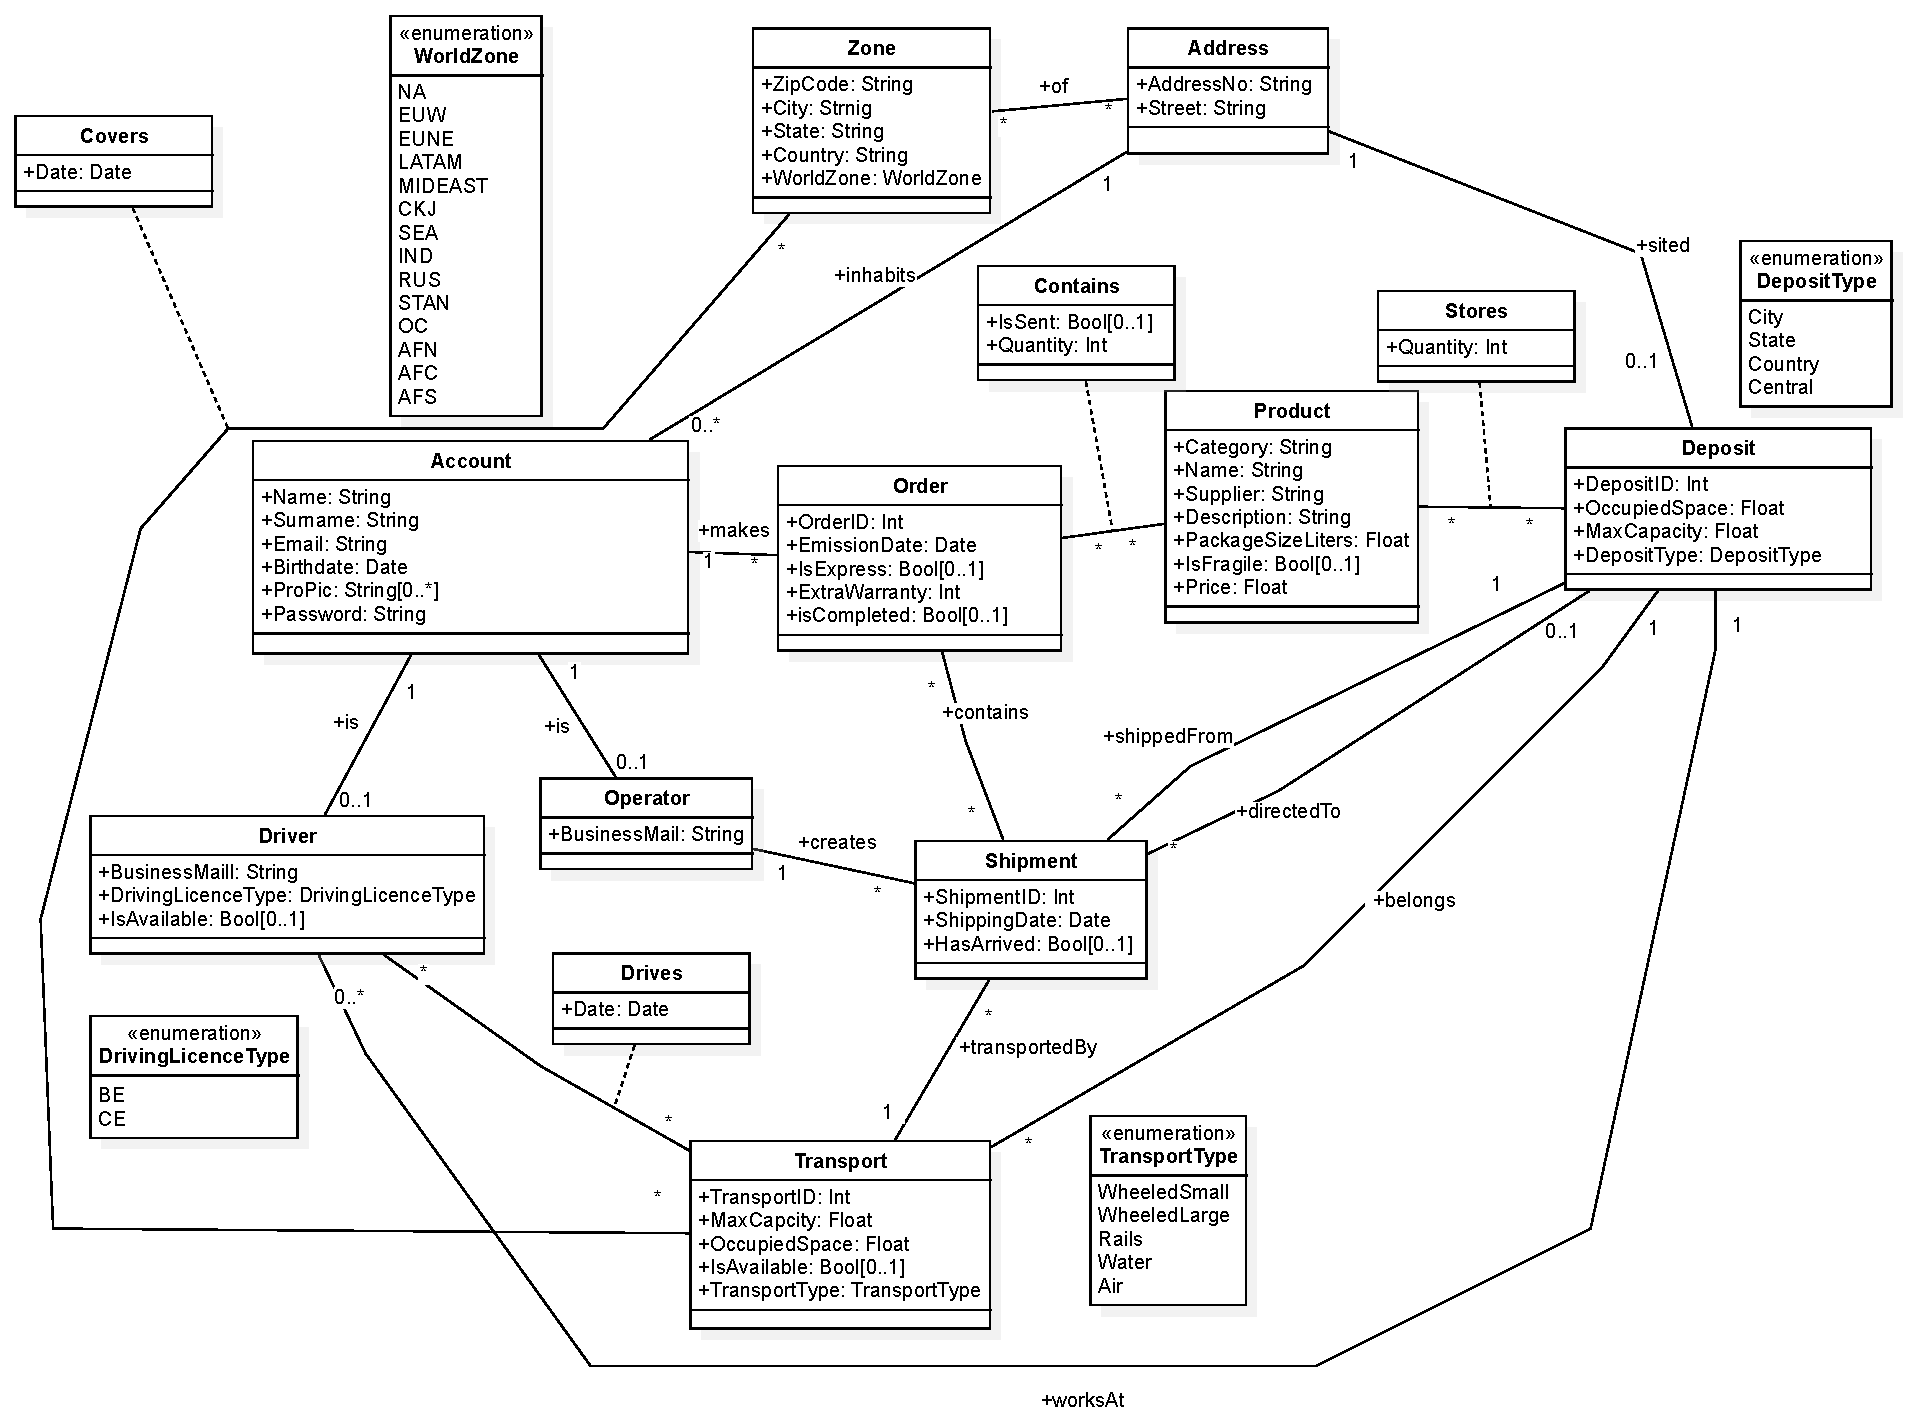
\includegraphics[width=\textwidth]{UML_Class_Diagram_Restructured.pdf} 
% \end{center}

\newpage

\section{Dizionari}

\subsection{Dizionario delle Classi}

\customTable{cYY}[Dizionario delle classi Prima Parte]{\textbfB{Classe} & \textbfB{Descrizione} & \textbfB{Attributi}}{
  \textbf{Account} & Generico utente che utilizza il sistema per effettuare ordini. & 
  {\footnotesize 
  \textbf{Name:} (\textit{string}): Nome dell'utente;
  
  \textbf{Surname} (\textit{string}): Cognome dell'utente;
  
  \textbf{Email} (\textit{string}): Chiave Primaria. Email dell'utente;

  \textbf{Birthdate} (\textit{date}): Data di nascita dell'utente;

  \textbf{ProPic} (\textit{string}): Eventuale immagine profilo dell'utente;

  \textbf{Password} (\textit{string}): Password dell'utente;  
  }\\


  \textbf{Operator} & Account di un impiegato che si occupa di creare le spedizioni. &
  {\footnotesize
  \textbf{BusinessMail} (\textit{string}): Chiave Primaria. Email aziendale dell'operatore;
  }\\


  \textbf{Driver} & Account di un autista che si occupa di effettuare le consegne. &
  {\footnotesize
  \textbf{BusinessMail} (\textit{string}): Chiave Primaria. Email aziendale dell'autista;

  \textbf{DrivingLincenceType} (\textit{DrivingLincenceType}): Tipologia di patente dell'autista;

  \textbf{IsAvailable} (\textit{bool}): Indica se l'autista è disponibile o meno;
  }\\


  \textbf{Order} & Ordine effettuato da un utente. Può contenere più prodotti e può essere spedito in più spedizioni. &
  {\footnotesize
  \textbf{OrderID} (\textit{integer}): Chiave Surrogata. Identificativo dell'ordine;

  \textbf{EmissionDate} (\textit{date}): Data di emissione dell'ordine;

  \textbf{IsExpress} (\textit{bool}): Indica se l'ordine è espresso o meno;

  \textbf{ExtraWarranty} (\textit{bool}): Indica se è stata acquistata una garanzia extra o meno;

  \textbf{IsCompleted} (\textit{bool}): Indica se l'ordine è stato completato o meno;
  }\\


  \textbf{Shipment} & Singola spedizione partita da un deposito. Può contenere più ordini e può raggiungere a più utenti o a un deposito. &
  {\footnotesize
  \textbf{ShipmentID} (\textit{integer}): Chiave Surrogata. Identificativo della spedizione; 

  \textbf{ShippingDate} (\textit{date}): Data della spedizione;
  }\\  
}

\newpage

\customTable{cYY}[Dizionario delle classi Seconda Parte]{\textbfB{Classe} & \textbfB{Descrizione} & \textbfB{Attributi}}{
  \textbf{Product} & Prodotto acquistabile da un utente. Può essere conservato in più depositi. &
  { \footnotesize
    \textbf{Type} (\textit{string}): Categoria del prodotto;

    \textbf{Name} (\textit{string}): Chiave Primaria. Nome del prodotto;

    \textbf{Supplier} (\textit{string}): Chiave Primaria. Fornitore del prodotto. Di default è \textit{UninaDelivery};
  
    \textbf{Description} (\textit{string}): Descrizione del prodotto;

    \textbf{PackageSizeLiters} (\textit{float}): Dimensione del prodotto in litri;

    \textbf{IsFagile} (\textit{bool}): Indica se il prodotto è fragile o meno;

    \textbf{Price} (\textit{float}): Prezzo del prodotto;
  }\\


  \textbf{Deposit} & Deposito per la conservazione di prodotti. Può contenere più prodotti e può essere raggiunto da più spedizioni. &
  {\footnotesize
  \textbf{DepositID} (\textit{integer}): Chiave Surrogata. Identificativo del deposito;

  \textbf{OccupiedSpace} (\textit{float}): Spazio del deposito attualmente occupato;

  \textbf{MaxCapacity} (\textit{float}): Spazio massimo del deposito;

  \textbf{DepositType} (\textit{DepositType}): Tipologia del deposito;
  }\\
  

  \textbf{Zone} & Zona del mondo raggiungibile da un mezzo di trasporto. Contiene più indirizzi. &
  {\footnotesize
  \textbf{ZipCode} (\textit{string}): Chiave Primaria. Codice di Avviamento Postale della zona;

  \textbf{City} (\textit{string}): Città in cui si trova la zona;

  \textbf{Country} (\textit{string}): Chiave Primaria. Paese in cui si trova la zona;
  
  \textbf{WorldZone} (\textit{string}): Zona del mondo in cui si trova la zona;
  }\\

  \textbf{Address} & Indirizzo di un utente o di un deposito. & 
  {\footnotesize

  \textbf{AddressNo} (\textit{string}): Chiave Primaria. Numero civico dell'indirizzo; 

  \textbf{Street} (\textit{string}): Via dell'indirizzo;
  }\\

  \textbf{Transport} & Mezzo di trasporto utilizzato per le spedizioni. & 
  {\footnotesize
  \textbf{TransportID} (\textit{integer}): Chiave Surrogata. Identificativo del mezzo di trasporto;

  \textbf{MaxCapacity} (\textit{float}): Capacità massima del mezzo di trasporto;

  \textbf{OccupiedSpace} (\textit{float}): Spazio attualmente occupato dal mezzo di trasporto;

  \textbf{IsAvailable} (\textit{bool}): Indica se il mezzo di trasporto è disponibile o meno. Il campo sarà valorizzato a \textit{true} solo se il mezzo non è già in viaggio;
  
  \textbf{TransportType} (\textit{TransportType}): Tipologia del mezzo di trasporto;
  }\\

}

\newpage
\subsection{Dizionario delle Associazioni}

\customTable{cYYY}[Dizionario delle associazioni Prima Parte]{\textbfB{Associazione} & \textbfB{Descrizione} & \textbfB{Attributi} & \textbfB{Classi Coinvolte}}{
  Val 1 & Val 2 & Val 3 & Val 4 \\
  Val 1.2 & Val 2.2 & Val 3.2 & Val 4.2 \\
}
  

\newpage
\subsection{Dizionario dei Vincoli}

\customTable{ccY}[Dizionario dei vincoli Prima Parte]{\textbfB{Vincolo} & \textbfB{Tipologia} & \textbfB{Descrizione}}{
  Val 1 & Val 2 & Val 3 \\
  Val 1.2 & Val 2.2 & Val 3.2 \\
}




% TODO: @RiccardoElena @zGenny write this section
  % it should contains:
  % [x] all the considerations about the UML diagram
  % [x] the changes made to the UML diagram
  % [ ] the new UML diagram
  % [ ] constrints dictonary (table (?)). Styled as the example in the slides

  % Chapter 3 - "Funzionalità"
  \chapter{Schema Logico}

\section{Traduzione delle Associazioni}

\customTable{cY}[Dizionario delle classi Seconda Parte]{\textbfB{Associazione} & \textbfB{Strategia di Traduzione}}{
  \textbf{makes} & {\footnotesize Migrazione della \underline{chiave primaria} di \textbf{Account} in \textbf{Order}.} \\
  \textbf{contains} & {\footnotesize Migrazione della \underline{chiave primaria} di \textbf{Product} in \textbf{Order}.} \\
  \textbf{stores} & {\footnotesize Definizione di una nuova tabella \textbf{Stores} con chiavi esterne verso \textbf{Product} e \textbf{Deposit}, oltre che gli attributi della relazione.} \\
  \textbf{worksAt} & {\footnotesize Migrazione della \underline{chiave primaria} di \textbf{Deposit} in \textbf{Driver}.} \\
  \textbf{belongs} & {\footnotesize Migrazione della \underline{chiave primaria} di \textbf{Deposit} in \textbf{Transport}.} \\
  \textbf{drives} & {\footnotesize Definizione di una nuova tabella \textbf{Drives} con chiavi esterne verso \textbf{Transport} e \textbf{Driver}, oltre che gli attributi della relazione.} \\
  \textbf{transportedBy} & {\footnotesize Migrazione della \underline{chiave primaria} di \textbf{Transport} in \textbf{Shipment}.} \\
  \textbf{covers} & {\footnotesize Definizione di una nuova tabella \textbf{Covers} con chiavi esterne verso \textbf{Transport} e \textbf{Area}, oltre che gli attributi della relazione.} \\
  \textbf{ships} & {\footnotesize Definizione di una nuova tabella \textbf{Ships} con chiavi esterne verso \textbf{Shipment} e \textbf{Order}.} \\
  \textbf{shippedFrom} & {\footnotesize Migrazione della \underline{chiave primaria} di \textbf{Deposit} in \textbf{Shipment}.} \\
  \textbf{shippedTo} & {\footnotesize Migrazione della \underline{chiave primaria} di \textbf{Deposit} in \textbf{Shipment}.} \\
  \textbf{is} & {\footnotesize Migrazione della \underline{chiave primaria} di \textbf{Account} in \textbf{Operator}.} \\
  \textbf{is} & {\footnotesize Migrazione della \underline{chiave primaria} di \textbf{Account} in \textbf{Driver}.} \\
  \textbf{inhabits} & {\footnotesize Migrazione della \underline{chiave primaria} di \textbf{Address} in \textbf{Account}.} \\
  \textbf{sited} & {\footnotesize Accorpamento delle classi coinvolte nella classe \textbf{Deposit}.}\\
  \textbf{located} & {\footnotesize Migrazione della \underline{chiave primaria} di \textbf{Address} in \textbf{Area}.} \\
}

\section{Traduzione delle Classi}

\subsection{Considerazioni sulla Traduzione delle Classi}

Per quanto riguarda l'individuazione delle chiavi primarie, ciò è stato già fatto nella sezione \intlink{individuazioneDelleChiaviPrimarie}{identificazione delle chiavi primarie}.

Dalla \textbf{traduzione delle associazioni} si è evidenziato come, per via delle strategie utilizzate per la traduzione, la classe \textbf{Address} sia ridondante. Infatti la classe \textbf{Deposit} e la classe \textbf{Account} ne contengono tutti i campi, essendo tutti chiavi primarie, e per la classe \textbf{Area} la migrazione delle chiavi avveniva \textit{verso \textbf{Address}}, diventando anch'esse chiavi primarie e venendo ereditate da \textbf{Deposit} e \textbf{Account}.
È sufficiente quindi per eliminare la classe \textbf{Address} oltre alle strategie già messe in atto durante la \textbf{traduzione delle associazioni} migrare le chiavi primarie di \textbf{Area} direttamente verso \textbf{Deposit} e \textbf{Account}, andando a diminuire l'overhead e risolvendo in automatico vincoli come \intlink{isAddressForSomethingGeneral}{\textbf{isAddressForSomethingGeneral}}.

Per mantenere la consistenza del database, va anche introdotto un vincolo di unicità nella nuova classe accorpata \textbf{Deposit}. Per garantire l'associazione di tipo \(1:1\) tra \textbf{Deposit} e \textbf{Address} è necessario che la quadrupla di campi \textit{AddressNo}, \textit{Street}, \textit{ZipCode} e \textit{Country} sia unica nella tabella.
\section{Schema Logico}

\begin{note}[Indicazioni di Chiave Primaria e Chiave Esterna]
  Per evidenziare la presenza di \textbf{chiavi primarie} e \textbf{chiavi esterne} nei diagrammi, si è deciso sottolineare le \underline{chiavi primarie} e mettere in corsivo le \textit{chiavi esterne}.

  Per evitare superflue verbosità si è scelto di chiamare tutti i campi che rappresentano una chiave esterna con il nome della chiave primaria cui fanno riferimento. In caso di ambiguità, si è scelto di utilizzare il nome dell'associazione tradotta con l'uso di tale chiave o la classe a cui appartiene la chiave primaria a cui fa riferimento la chiave esterna.
\end{note}


\customTableLogic{|Y|Y|Y|Y|Y|}{5}{Area}{
  \underline{ZipCode} & City & State & \underline{Country} & WorldZone
}

\customTableLogic{|Y|Y|Y|Y|Y|}{5}{Account}{
  Name & Surname & \underline{Email} & Birthdate & ProPic \\
  \hline
  Password & \textit{AddressNo} & \textit{Street} & \textit{ZipCode} & \textit{Country}
}
% TODO: @zGenny 
\customTableLogic{|Y|Y|Y|Y|Y|}{5}{Order}{
  \underline{OrderID} & EmissionDate & isExpress & ExtraWarranty & IsCompleted \\
  \hline
  \textit{Email} & \textit{Quantity} & \textit{Name} & \textit{Supplier} & - 
}

\customTableLogic{|Y|Y|Y|Y|}{4}{Product}{
  Category & \underline{Name} & \underline{Supplier} & Description \\
  \hline
  PackageSizeLiters & isFragile & Price & ---
}

\customTableLogic{|Y|Y|Y|Y|}{4}{Stores}{
  \textit{Name} & \textit{Supplier} & \textit{DepositID} & Quantity
}

\customTableLogic{|Y|Y|Y|Y|}{4}{Deposit}{
  \underline{DepositID} & OccupiedSpace & MaxCapacity & DepositType \\
  \hline
  \textit{AddressNo} & \textit{Street} & \textit{ZipCode} & \textit{Country}
}

\customTableLogic{|Y|Y|Y|Y|}{4}{Shipment}{
  \underline{ShipmentID} & ShippingDate & HasArrived & \textit{ShippedFrom} \\
  \hline
  \textit{DirectedTo} & \textit{BusinessMail} & \textit{TransportID} & ---
}

\customTableLogic{|Y|Y|}{2}{Ships}{
  \textit{ShipmentID} & \textit{OrderID}
}

\customTableLogic{|Y|Y|}{2}{Operator}{
  \underline{BusinessMail} & \textit{Email}
}

\customTableLogic{|Y|Y|Y|}{3}{Transport}{
  \underline{TransportID} & MaxCapacity & OccupiedSpace \\
  \hline IsAvailable & TransportType & \textit{DepositID}
}

\customTableLogic{|Y|Y|Y|}{3}{Drives}{
  \textit{TransportID} & \textit{BusinessMail} & Date
}

\customTableLogic{|Y|Y|Y|}{3}{Driver}{
  \underline{BusinessMail} & DrivingLincenceType & IsAvailable \\
  \hline
  \textit{Email} & \textit{DepositID} & ---
}

\customTableLogic{|Y|Y|Y|Y|}{4}{Covers}{
  \textit{TransportID} & \textit{ZipCode} & \textit{Country} & Date
}


  % Chapter 4 - "Mockups"
  \chapter{Implementazione delle Tabelle}

In conclusione si riportano le istruzioni per l'implementazione fisica del database.

Come DBMS provider si è scelto di utilizzare PostgreSQL, per la sua facilità di utilizzo e la sua affidabilità.

Il database è hostato localmente per rendere più agevole la connessione.

Per pulizia del codice si è preferito lavorare su uno \textbf{schema} creato appositamente per il progetto, chiamato \textbf{UninaDelivery}.

\section{Definizione dei Domini Personalizzati}

Vista la vasta gamma di vincoli di dominio simili su vari campi, si è deciso di definire dei domini personalizzati per facilitare la creazione delle tabelle.

\begin{lstlisting}
  CREATE DOMAIN letterString AS text CHECK (VALUE ~ '^[a-zA-Z]+$');
  
  CREATE DOMAIN numericString AS text CHECK (VALUE ~ '^[0-9]+$');
  
  CREATE DOMAIN alphanumericString AS text CHECK (VALUE ~ '^\w+[\w\s.]$');
  
  CREATE DOMAIN emailString AS text CHECK (
    VALUE ~ '^\w+[\w.]*\w@[a-zA-Z.]+\.[a-zA-Z]{2,}$'
  );
\end{lstlisting}

Inoltre per i campi che nel diagramma ristrutturato sono stati definiti come \textbf{enumerazioni}, si è deciso di utilizzare dei tipi enumerati personalizzati.

\begin{lstlisting}
  CREATE TYPE WorldZone AS ENUM (
    'NA', 'EUW', 'EUNE', 'LATAM', 'MIDEAST', 'CKJ', 'SEA', 'IND', 'RUS', 'STAN', 
    'OC', 'AFN', 'AFC', 'AFS'
  );

  CREATE TYPE DepositType AS ENUM (
    'City', 'State', 'Country', 'Central'
  );

  CREATE TYPE TransportType AS ENUM (
    'WheeledSmall', 'WheeledLarge', 'Rails', 'Water', 'Air'
  );
  
  CREATE TYPE DrivingLicenceType AS ENUM ('BE', 'CE');
\end{lstlisting}

\section{Creazione delle Tabelle}

Vediamo ora la creazione delle tabelle, con annessi vincoli di dominio e di n-upla, oltre che le chiavi primarie e le chiavi esterne.

\begin{lstlisting}[caption={Creazione della tabella \textbf{Area}}]
  CREATE TABLE Area (
    ZipCode numericString NOT NULL,
    City letterString NOT NULL,
    State letterString NOT NULL,
    Country letterString NOT NULL,
    WorldZone WorldZone NOT NULL
  );
  ALTER TABLE Area ADD CONSTRAINT Area_pk PRIMARY KEY (ZipCode, Country);
\end{lstlisting}

\begin{lstlisting}[caption={Creazione della tabella \textbf{Account}}]
  CREATE TABLE Account (
    Name letterString NOT NULL,
    Surname letterString NOT NULL,
    Email emailString NOT NULL,
    Birthdate date NOT NULL,
    ProPic text,
    Password text NOT NULL,
    AddressNo alphNumString NOT NULL,
    Street alphNumString NOT NULL,
    ZipCode numericString NOT NULL,
    Country letterString NOT NULL
  );
  ALTER TABLE account ADD CONSTRAINT Account_pk PRIMARY KEY (Email);
  ALTER TABLE account ADD CONSTRAINT validAccountBirthdate CHECK (
    EXTRACT( YEAR FROM age(Birthdate)) >= 16 
  );
  ALTER TABLE account ADD CONSTRAINT formatAccountPassword CHECK(
    Password ~ '^[A-Fa-f0-9]{64}$'
  );
  ALTER TABLE account ADD CONSTRAINT formatAccountProPic CHECK (
    ProPic ~ '^\/9j\/4AAQSkZJRg[-A-Za-z0-9+\/]*={0,2}$'
  );
  ALTER TABLE Account ADD CONSTRAINT formatAccountAddressNo CHECK (
    AddressNo ~ '^[1-9]\d*[a-z]?(?:BIS)?$'
  );
  ALTER TABLE Account ADD CONSTRAINT account_fk FOREIGN KEY (ZipCode, Country) REFERENCES Area(ZipCode, Country) ON DELETE CASCADE ON UPDATE CASCADE;
\end{lstlisting}
  

\newpage
\begin{lstlisting}[caption={Creazione della tabella \textbf{Order}}]
  CREATE TABLE "Order"(
    OrderID SERIAL, 
    EmissionDate Date NOT NULL,
    IsExpress boolean,
    ExtraWarranty smallint NOT NULL,
    IsCompleted boolean,
    Email emailString,
    Quantity integer NOT NULL
  );
  ALTER TABLE "Order" ADD CONSTRAINT Order_pk PRIMARY KEY (OrderID);
  ALTER TABLE "Order" ADD CONSTRAINT formatOrderExtraWarranty CHECK (
    ExtraWarranty >=0
  );
  ALTER TABLE "Order" ADD CONSTRAINT Order_fk FOREIGN KEY (Email) REFERENCES Account(Email) ON DELETE SET NULL ON UPDATE CASCADE;
  ALTER TABLE "Order" ADD CONSTRAINT formatOrderEmissionDate CHECK (
    EmissionDate <= current_date
  );
  ALTER TABLE "Order" ADD CONSTRAINT formatOrderQuantity CHECK (
    Quantity > 0
  );
\end{lstlisting}

\begin{lstlisting}[caption={Creazione della tabella \textbf{Stores}}]
  CREATE TABLE Stores(
    Name text NOT NULL,
    Supplier text NOT NULL,
    DepositID integer NOT NULL,
    Quantity integer NOT NULL
  );
  ALTER TABLE Stores ADD CONSTRAINT noDuplicateProductInDeposit UNIQUE (Name, Supplier, DepositID);
  ALTER TABLE Stores ADD CONSTRAINT Stores_fk_Product FOREIGN KEY (Name, Supplier) REFERENCES Product(Name, Supplier) ON DELETE CASCADE ON UPDATE CASCADE;
  ALTER TABLE Stores ADD CONSTRAINT Stores_fk_Deposit FOREIGN KEY (DepositID) REFERENCES Deposit(DepositID) ON DELETE CASCADE ON UPDATE CASCADE;
  ALTER TABLE Stores ADD CONSTRAINT formatStoresQuantity CHECK(Quantity > 0);
\end{lstlisting}

\newpage

\begin{lstlisting}[caption={Creazione della tabella \textbf{Deposit}}]
  CREATE TABLE Deposit (
    DepositID SERIAL NOT NULL,
    OccupiedSpace real NOT NULL DEFAULT 0,
    MaxCapacity real NOT NULL,
    DepositType DepositType NOT NULL,
    AddressNo alphNumString NOT NULL,
    Street alphNumString NOT NULL,
    ZipCode numericString NOT NULL,
    Country letterString NOT NULL
  );
  ALTER TABLE Deposit ADD CONSTRAINT Deposit_pk PRIMARY KEY ( DepositID);
  ALTER TABLE Deposit ADD CONSTRAINT foramtDepositOccupiedSpace CHECK(
    OccupiedSpace >= 0
  );
  ALTER TABLE Deposit ADD CONSTRAINT foramtDepositMaxCapacity CHECK(
    MaxCapacity > 0
  );
  ALTER TABLE Deposit ADD CONSTRAINT checkDepositFullness CHECK (
    OccupiedSpace <= MaxCapacity
  );
  ALTER TABLE Deposit ADD CONSTRAINT formatDepositAddressNo CHECK (
    AddressNo ~ '^[1-9]\d*[a-z]?(?:BIS)?$'
  );
  ALTER TABLE Deposit ADD CONSTRAINT Deposit_fk FOREIGN KEY (ZipCode, Country) REFERENCES Area(ZipCode, Country) ON DELETE CASCADE ON UPDATE CASCADE;
  ALTER TABLE deposit ADD CONSTRAINT onlyOneDepositPerAddress UNIQUE(AddressNo, Street, ZipCode, Country);
\end{lstlisting}

\newpage

\begin{lstlisting}[caption={Creazione della tabella \textbf{Product}}]
  CREATE TABLE Product (
    Category letterString NOT NULL,
    Name text NOT NULL,
    Supplier text NOT NULL,
    Description text NOT NULL,
    PackageSizeLiters real NOT NULL,
    IsFragile boolean,
    Price numeric(100,2)
  );
  ALTER TABLE Product ADD CONSTRAINT Product_pk PRIMARY KEY (Name,Supplier);
  ALTER TABLE Product ADD CONSTRAINT formatProductName CHECK(
    Name ~ '^[a-zA-Z0-9]+[\ a-zA-Z0-9!@#$%^&*()_+{}\[\]:;<>,.?''~\\\/-]*$'
  );
  ALTER TABLE Product ADD CONSTRAINT formatProductDescription CHECK(
    Description ~ '^[a-zA-Z0-9]+[\ a-zA-Z0-9!@#$%^&*()_+{}\[\]:;<>,.?''~\\\/-]*$'
  );
  ALTER TABLE Product ADD CONSTRAINT formatProductSupplier CHECK(
    Supplier ~ '^[a-zA-Z0-9]+[\ a-zA-Z0-9!@#$%^&*()_+{}\[\]:;<>,.?''~\\\/-]*$'
  );
  ALTER TABLE Product ADD CONSTRAINT formatProductPackageSizeLiters CHECK(
    PackageSizeLiters > 0
  );
  ALTER TABLE Product ADD CONSTRAINT formatProductPrice CHECK(
    Price > 0
  );
  ALTER TABLE Product ADD CONSTRAINT checkProductDescriptionOnTopic CHECK(
    (Description ILIKE ('% ' || Name || '%')) AND 
    (Description ILIKE ('% ' || Supplier || '%'))
  )
\end{lstlisting}

\begin{lstlisting}[caption={Creazione della tabella \textbf{Covers}}]
  CREATE TABLE Covers (
    TransportID integer NOT NULL,
    ZipCode numericString NOT NULL,
    Country letterString NOT NULL,
    Date date NOT NULL,
    OccupiedSpace real NOT NULL DEFAULT 0
  );
  ALTER TABLE Covers ADD CONSTRAINT Covers_fk_Transport FOREIGN KEY (TransportID) REFERENCES Transport(TransportID) ON DELETE CASCADE ON UPDATE CASCADE;
  ALTER TABLE Covers ADD CONSTRAINT Covers_fk_Area FOREIGN KEY (ZipCode, Country) REFERENCES Area(ZipCode, Country) ON DELETE CASCADE ON UPDATE CASCADE;
  ALTER TABLE Covers ADD CONSTRAINT onlyOneAreaPerDay UNIQUE (TransportID, Date);
  ALTER TABLE Covers ADD CONSTRAINT formatCoversOccupiedSpace CHECK (
    OccupiedSpace >=0
  );
\end{lstlisting}

\newpage
\begin{lstlisting}[caption={Creazione della tabella \textbf{Transport}}]
  CREATE TABLE Transport (
    TransportID Serial NOT NULL,
    OccupiedSpace real NOT NULL DEFAULT 0,
    MaxCapacity real NOT NULL,
    IsAvailable boolean, 
    TransportType TransportType NOT NULL,
    DepositID integer NOT NULL
  );
  ALTER TABLE Transport ADD CONSTRAINT Transport_pk PRIMARY KEY(TransportID);
  ALTER TABLE Transport ADD CONSTRAINT Transport_fk FOREIGN KEY(DepositID) REFERENCES Deposit(DepositID) ON DELETE CASCADE ON UPDATE CASCADE; 
  ALTER TABLE Transport ADD CONSTRAINT formatTransportMaxCapacity CHECK (
    MaxCapacity >0
  );
  ALTER TABLE Transport ADD CONSTRAINT checkTransportFullness CHECK(
    OccupiedSpace <= MaxCapacity
  );
\end{lstlisting}

\begin{lstlisting}[caption={Creazione della tabella \textbf{Operator}}]
  CREATE TABLE Operator (
  Email emailString NOT NULL,
  BusinessMail emailString NOT NULL DEFAULT 'tobechanged@example.com'
);
ALTER TABLE Operator ADD CONSTRAINT Operator_pk PRIMARY KEY (BusinessMail);
ALTER TABLE Operator ADD CONSTRAINT Operator_fk FOREIGN KEY (Email) REFERENCES Account(Email) ON DELETE CASCADE ON UPDATE CASCADE;
\end{lstlisting}


\begin{lstlisting}[caption={Creazione della tabella \textbf{Ships}}]
  CREATE TABLE Ships ( 
    ShipmentID integer NOT NULL,
    OrderID integer NOT NULL
  );
  ALTER TABLE Ships ADD CONSTRAINT noDuplicateOrderInShipment UNIQUE (ShipmentID, OrderID);
  ALTER TABLE Ships ADD CONSTRAINT Ships_fk_Shipment FOREIGN KEY (ShipmentID) REFERENCES Shipment(ShipmentID) ON DELETE CASCADE ON UPDATE CASCADE;
  ALTER TABLE Ships ADD CONSTRAINT Ships_fk_Order FOREIGN KEY (OrderID) REFERENCES "Order"(OrderID) ON DELETE CASCADE ON UPDATE CASCADE;
\end{lstlisting}

\newpage
\begin{lstlisting}[caption={Creazione della tabella \textbf{Shipment}}]
  CREATE TABLE Shipment (
    ShipmentID Serial NOT NULL,
    ShippingDate date NOT NULL,
    HasArrived boolean,
    ShippedFrom integer NOT NULL,
    DirectedTo integer,
    BusinessMail emailString NOT NULL,
    TransportID integer NOT NULL
  );
  ALTER TABLE Shipment ADD CONSTRAINT Shipment_pk PRIMARY KEY (ShipmentID);
  ALTER TABLE Shipment ADD CONSTRAINT Shipment_fk_startDeposit FOREIGN KEY (ShippedFrom) REFERENCES Deposit(DepositID) ON DELETE CASCADE ON UPDATE CASCADE;
  ALTER TABLE Shipment ADD CONSTRAINT Shipment_fk_arrivalDeposit FOREIGN KEY (DirectedTo) REFERENCES Deposit(DepositID) ON DELETE CASCADE ON UPDATE CASCADE;
  ALTER TABLE shipment ADD CONSTRAINT onlyOneTravelPerDay UNIQUE ( ShippingDate, TransportID ) ;
  ALTER TABLE Shipment ADD CONSTRAINT checkDifferentStartEndDeposits CHECK (
    ShippedFrom <> DirectedTo
  );
  ALTER TABLE Shipment ADD CONSTRAINT validShipmentDate CHECK (
    ShippingDate >= current_date
  );
  ALTER TABLE Shipment ADD CONSTRAINT Shipment_fk_transport FOREIGN KEY (TransportID) REFERENCES Transport(TransportID) ON DELETE RESTRICT ON UPDATE CASCADE;
  ALTER TABLE Shipment ADD CONSTRAINT Shipment_fk_operator FOREIGN KEY (BusinessMail) REFERENCES Operator(Businessmail) ON DELETE CASCADE ON UPDATE CASCADE;
\end{lstlisting} 
 
\begin{lstlisting}[caption={Creazione della tabella \textbf{Driver}}]
  CREATE TABLE Driver (
    BusinessMail emailString NOT NULL DEFAULT 'tobechanged@example.com',
    DrivingLicenceType DrivingLicenceType NOT NULL,
    Email emailString, 
    DepositID integer NOT NULL 
  );
  ALTER TABLE Driver ADD CONSTRAINT Driver_pk PRIMARY KEY (BusinessMail);
  ALTER TABLE Driver ADD CONSTRAINT Driver_fk_Account FOREIGN KEY (Email) REFERENCES Account(Email) ON DELETE CASCADE ON UPDATE CASCADE;
  ALTER TABLE Driver ADD CONSTRAINT Driver_fk_Deposit FOREIGN KEY (DepositID) REFERENCES Deposit(DepositID) ON DELETE CASCADE ON UPDATE CASCADE;
\end{lstlisting}

\newpage

\begin{lstlisting}[caption={Creazione della tabella \textbf{Drives}}]
  CREATE TABLE Drives(
    TransportID integer NOT NULL,
    BusinessMail emailString NOT NULL,
    Date date NOT NULL
  );
  ALTER TABLE Drives ADD CONSTRAINT Drives_fk_Driver FOREIGN KEY (BusinessMail) REFERENCES Driver(BusinessMail) ON DELETE CASCADE ON UPDATE CASCADE;
  ALTER TABLE Drives ADD CONSTRAINT Drives_fk_Transport FOREIGN KEY (TransportID) REFERENCES Transport(TransportID) ON DELETE CASCADE ON UPDATE CASCADE;
  ALTER TABLE Drives ADD CONSTRAINT onlyOneTravelPerDayTransport UNIQUE (TransportID, Date);
  ALTER TABLE Drives ADD CONSTRAINT onlyOneTravelPerDayDriver UNIQUE (BusinessMail, Date);
\end{lstlisting}


\end{document}

